\chapter{Implementation Details and Results}
\label{chap:chap4}
\renewcommand{\arraystretch}{1.2}

In the current chapter, ....

\section{Section}

Text... In Table \ref{tab:datasets_used} ....

\begin{table*}[htb!]
    \caption[Caption.]{Caption.}
	\label{tab:datasets_used}    
    \centering
    \resizebox{1\textwidth}{!}{
    \begin{tabular}{c c c c c}
       \noalign{\hrule height 1.5pt}

    \multicolumn{1}{c}{\textbf{Dataset}}& \multicolumn{1}{c}{\textbf{Number of instances}}& \multicolumn{1}{c}{\textbf{Number of predictors}}&\multicolumn{1}{c}{\textbf{Numerical predictors}}&\multicolumn{1}{c}{\textbf{Categorical predictors}}\\
    \hline 
    A1 & 198 & 11 & 8 & 3 \\
    A2 & 198 & 11 & 8 & 3 \\
    A3 & 198 & 11 & 8 & 3 \\ 
    \noalign{\hrule height 1.5pt}%\hline
    \end{tabular}
    }
\end{table*}

Figure \ref{fig:boxplot_single} ...

\begin{figure}[!htb]
    \centering
    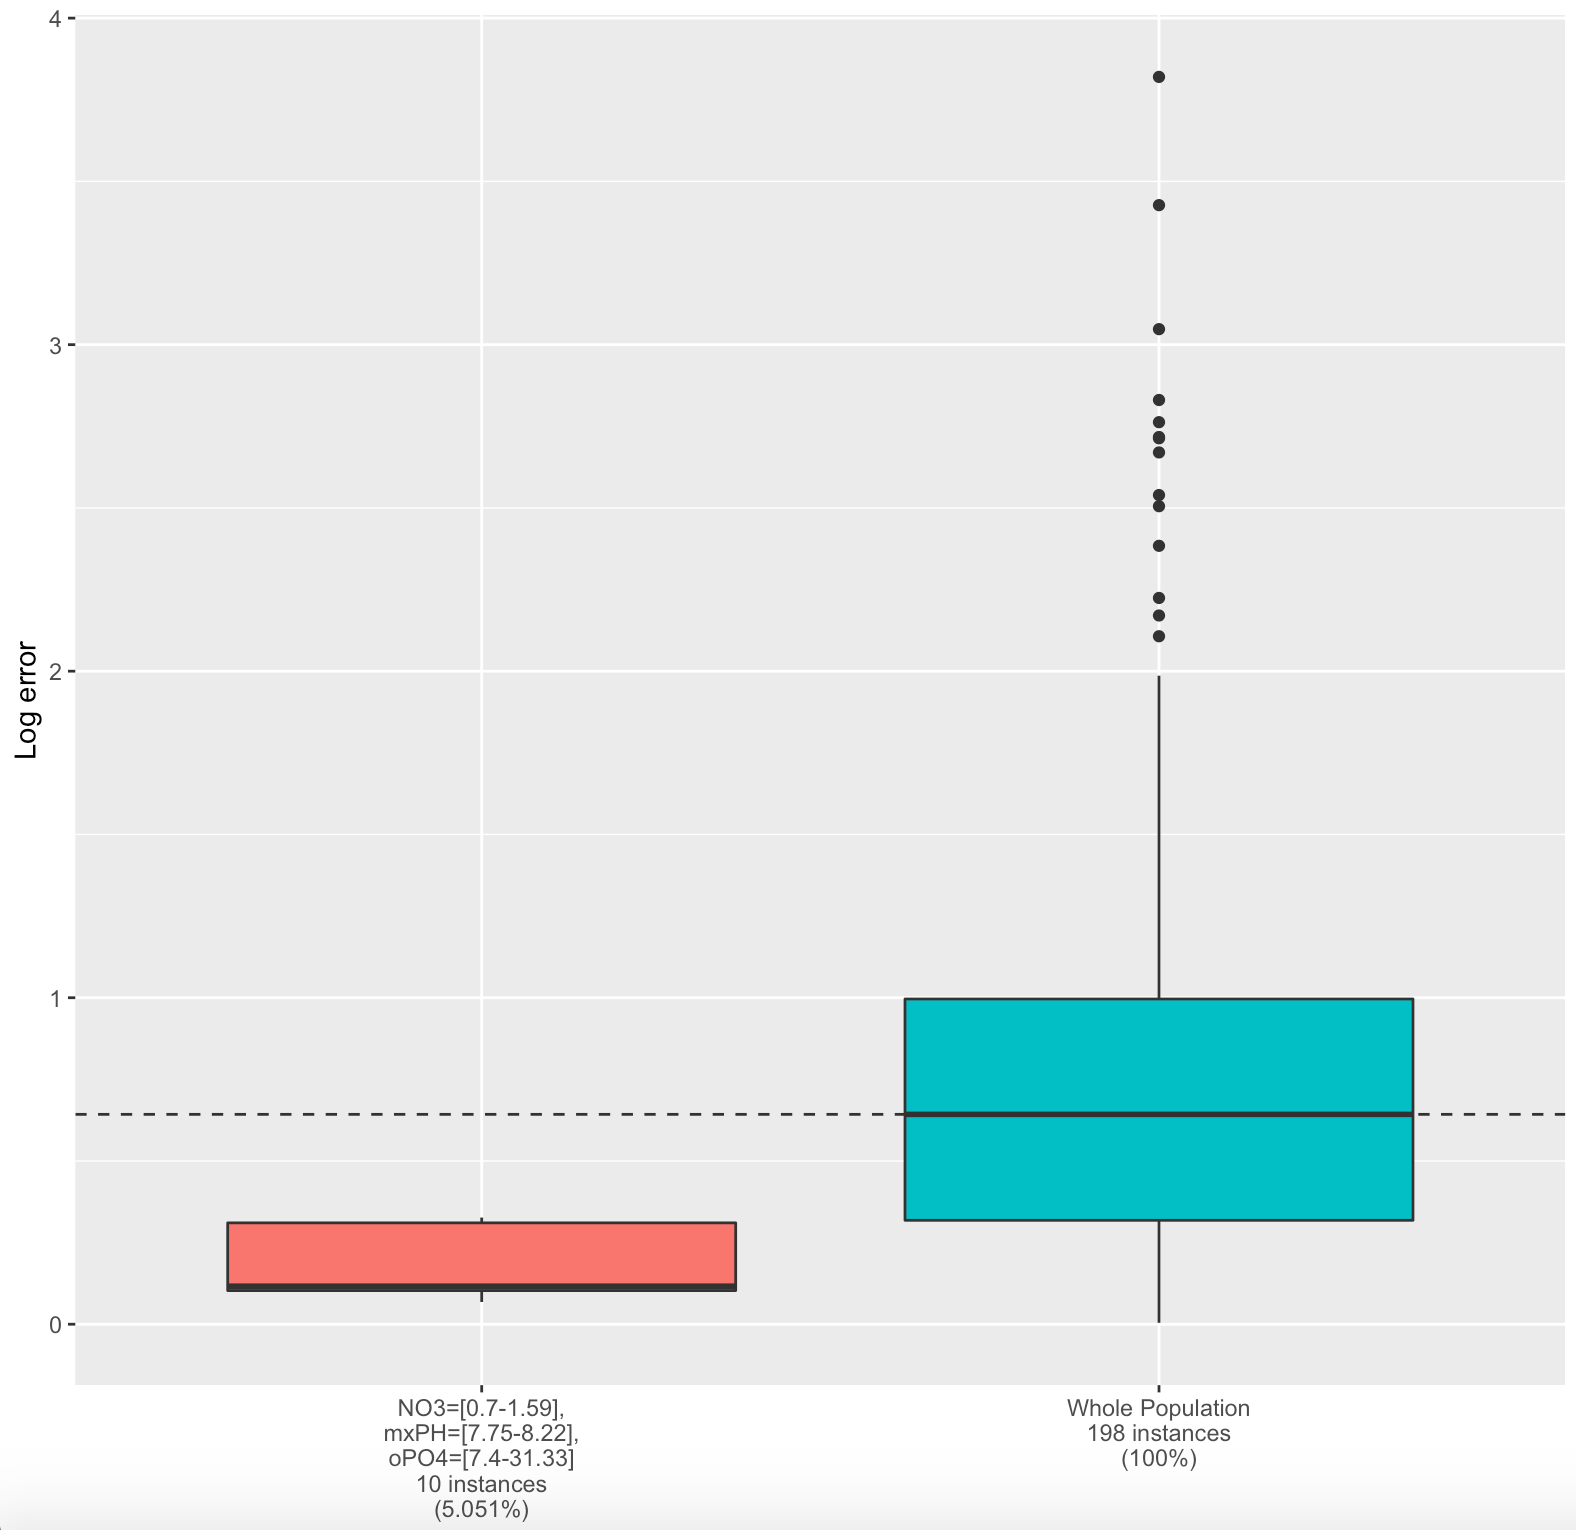
\includegraphics[width=0.45\textwidth]{/chpt_4/boxplot/single.png}
 	\caption[Caption.]
 	{Caption.}
 	\label{fig:boxplot_single}
\end{figure}

Figure \ref{fig:fig_2} contains an example of subfigures (Figure \ref{fig:subfigure_1}, ...).

\begin{figure}[!htb]
\centering
\imagewidth=0.32\textwidth
\captionsetup[subfigure]{width=0.8\imagewidth}
\begin{subfigure}{.32\textwidth}
  \centering
  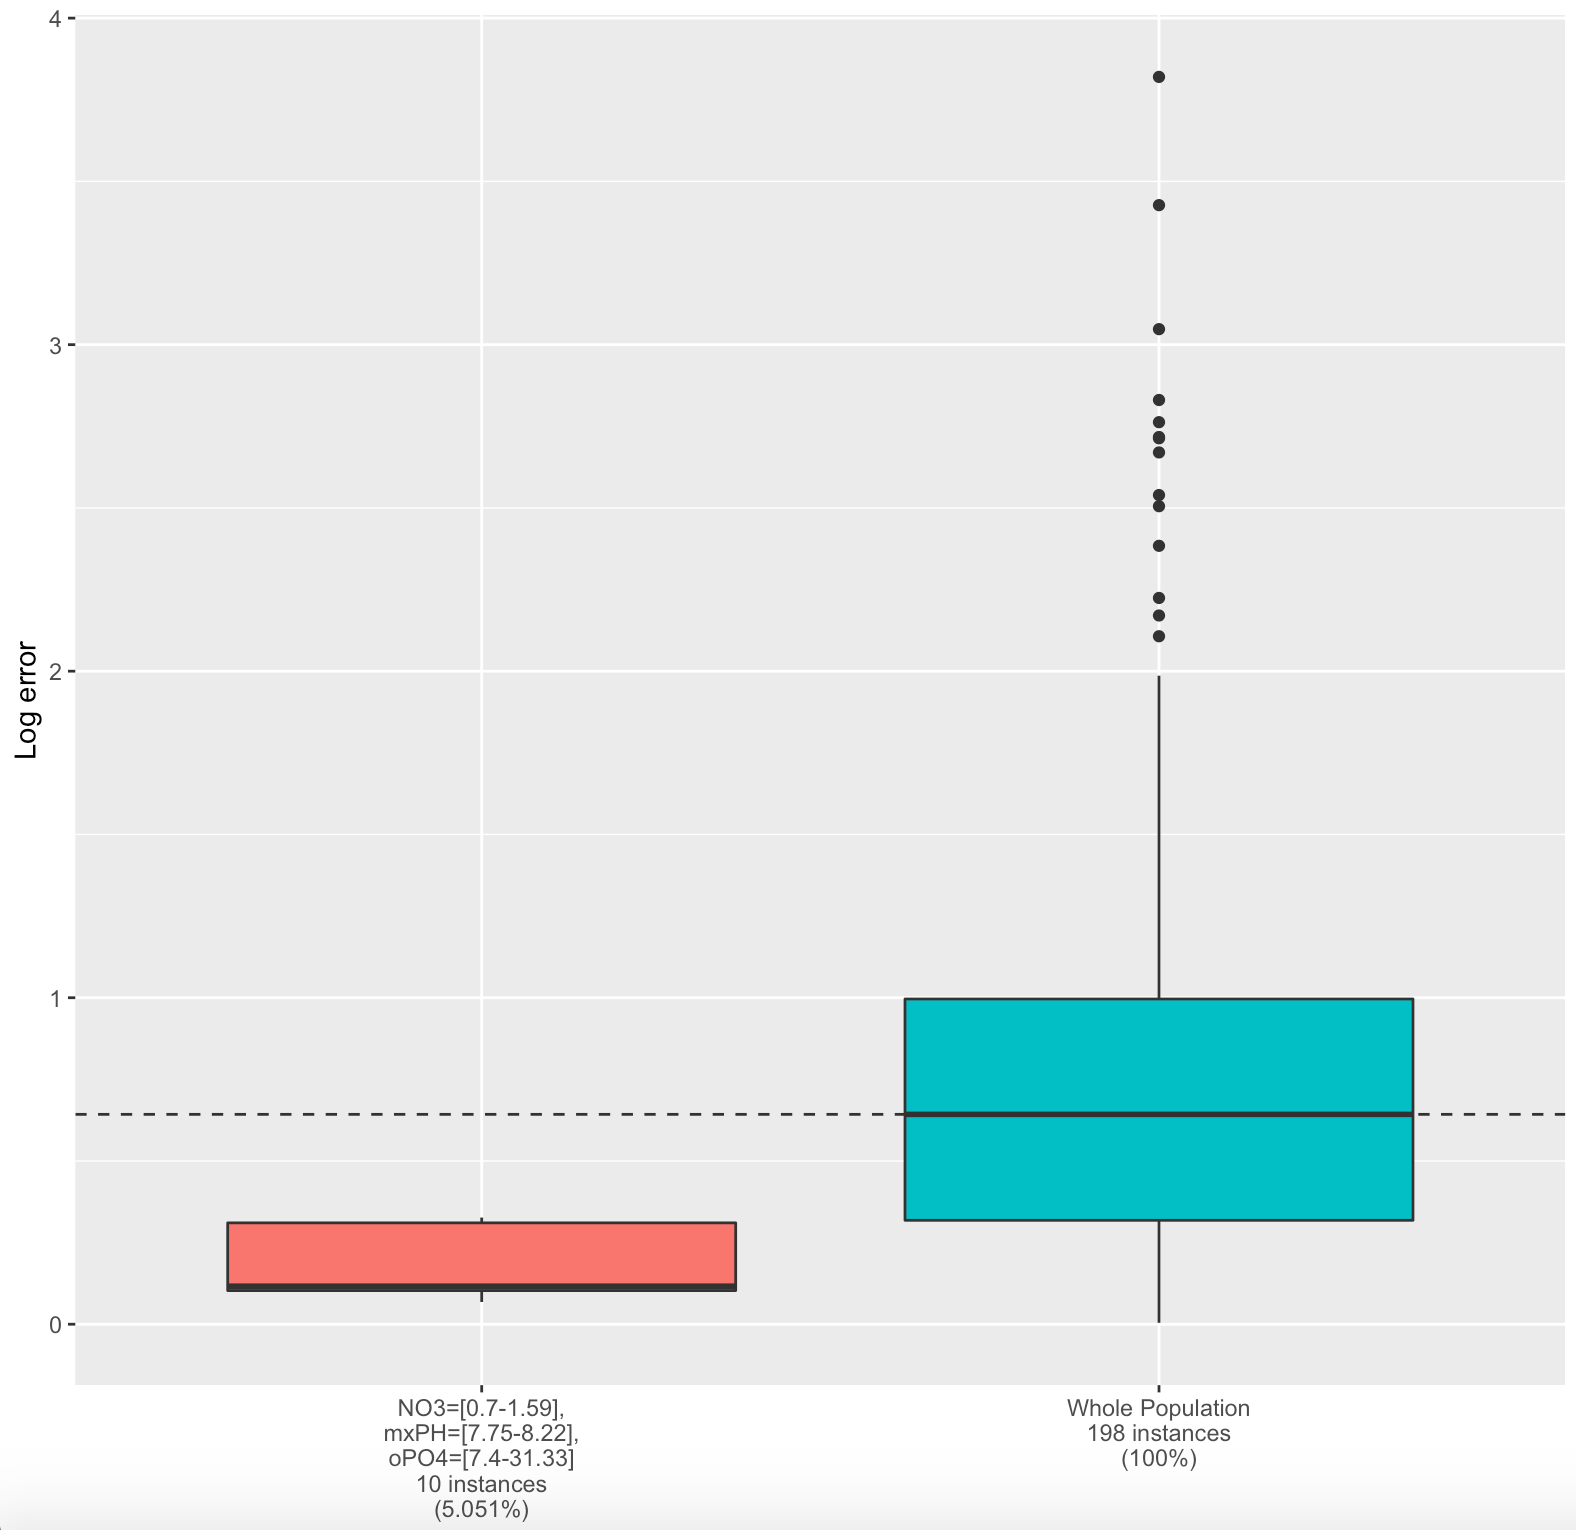
\includegraphics[width=0.97\linewidth]{/chpt_4/boxplot/single.png}
  \caption{Caption.}
  \label{fig:subfigure_1}
\end{subfigure}
\begin{subfigure}{.32\textwidth}
  \centering
  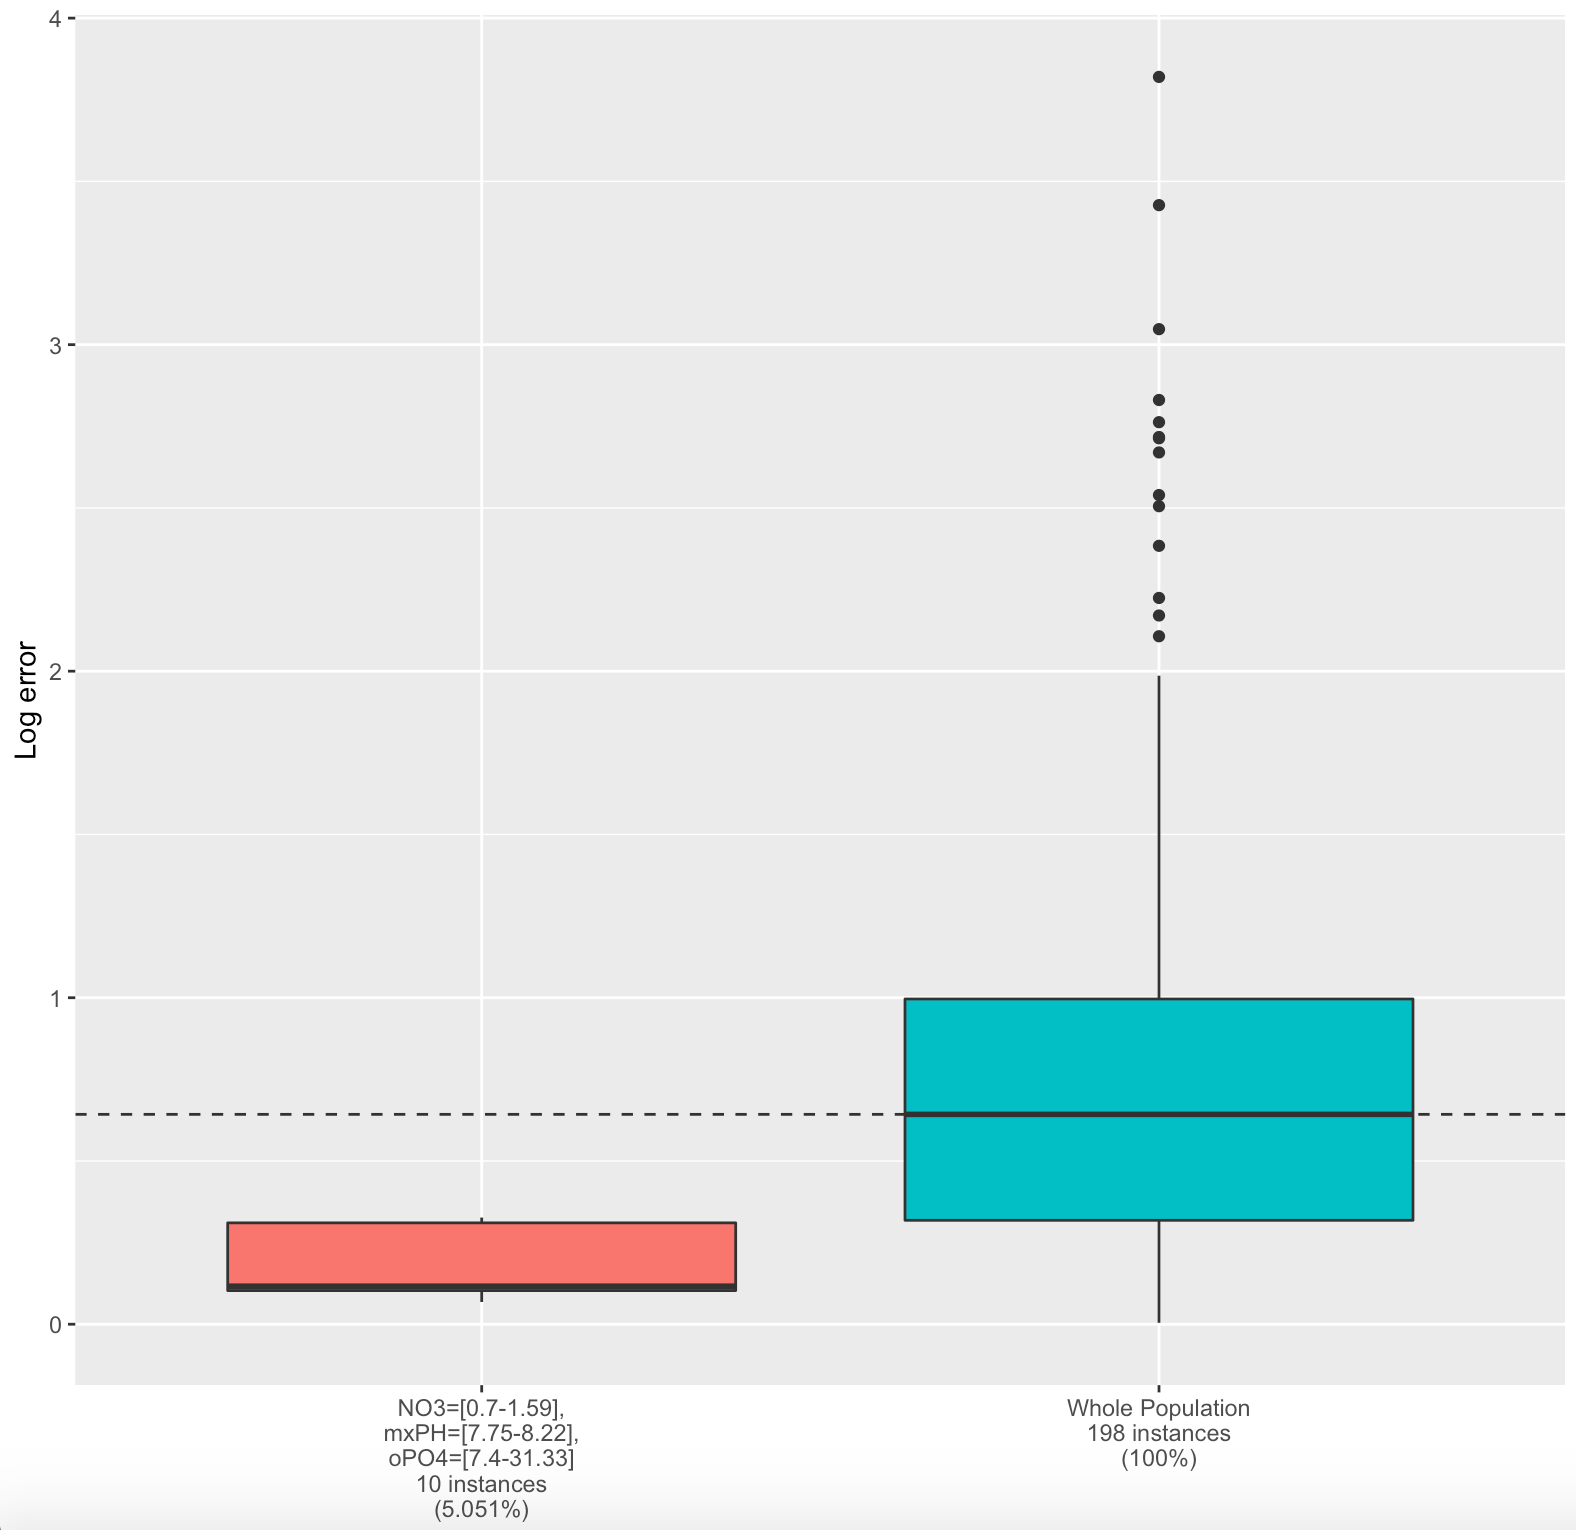
\includegraphics[width=0.97\linewidth]{/chpt_4/boxplot/single.png}
  \caption{Caption.} 
  \label{fig:subfigure_2}
\end{subfigure}
\begin{subfigure}{.32\textwidth}
  \centering
  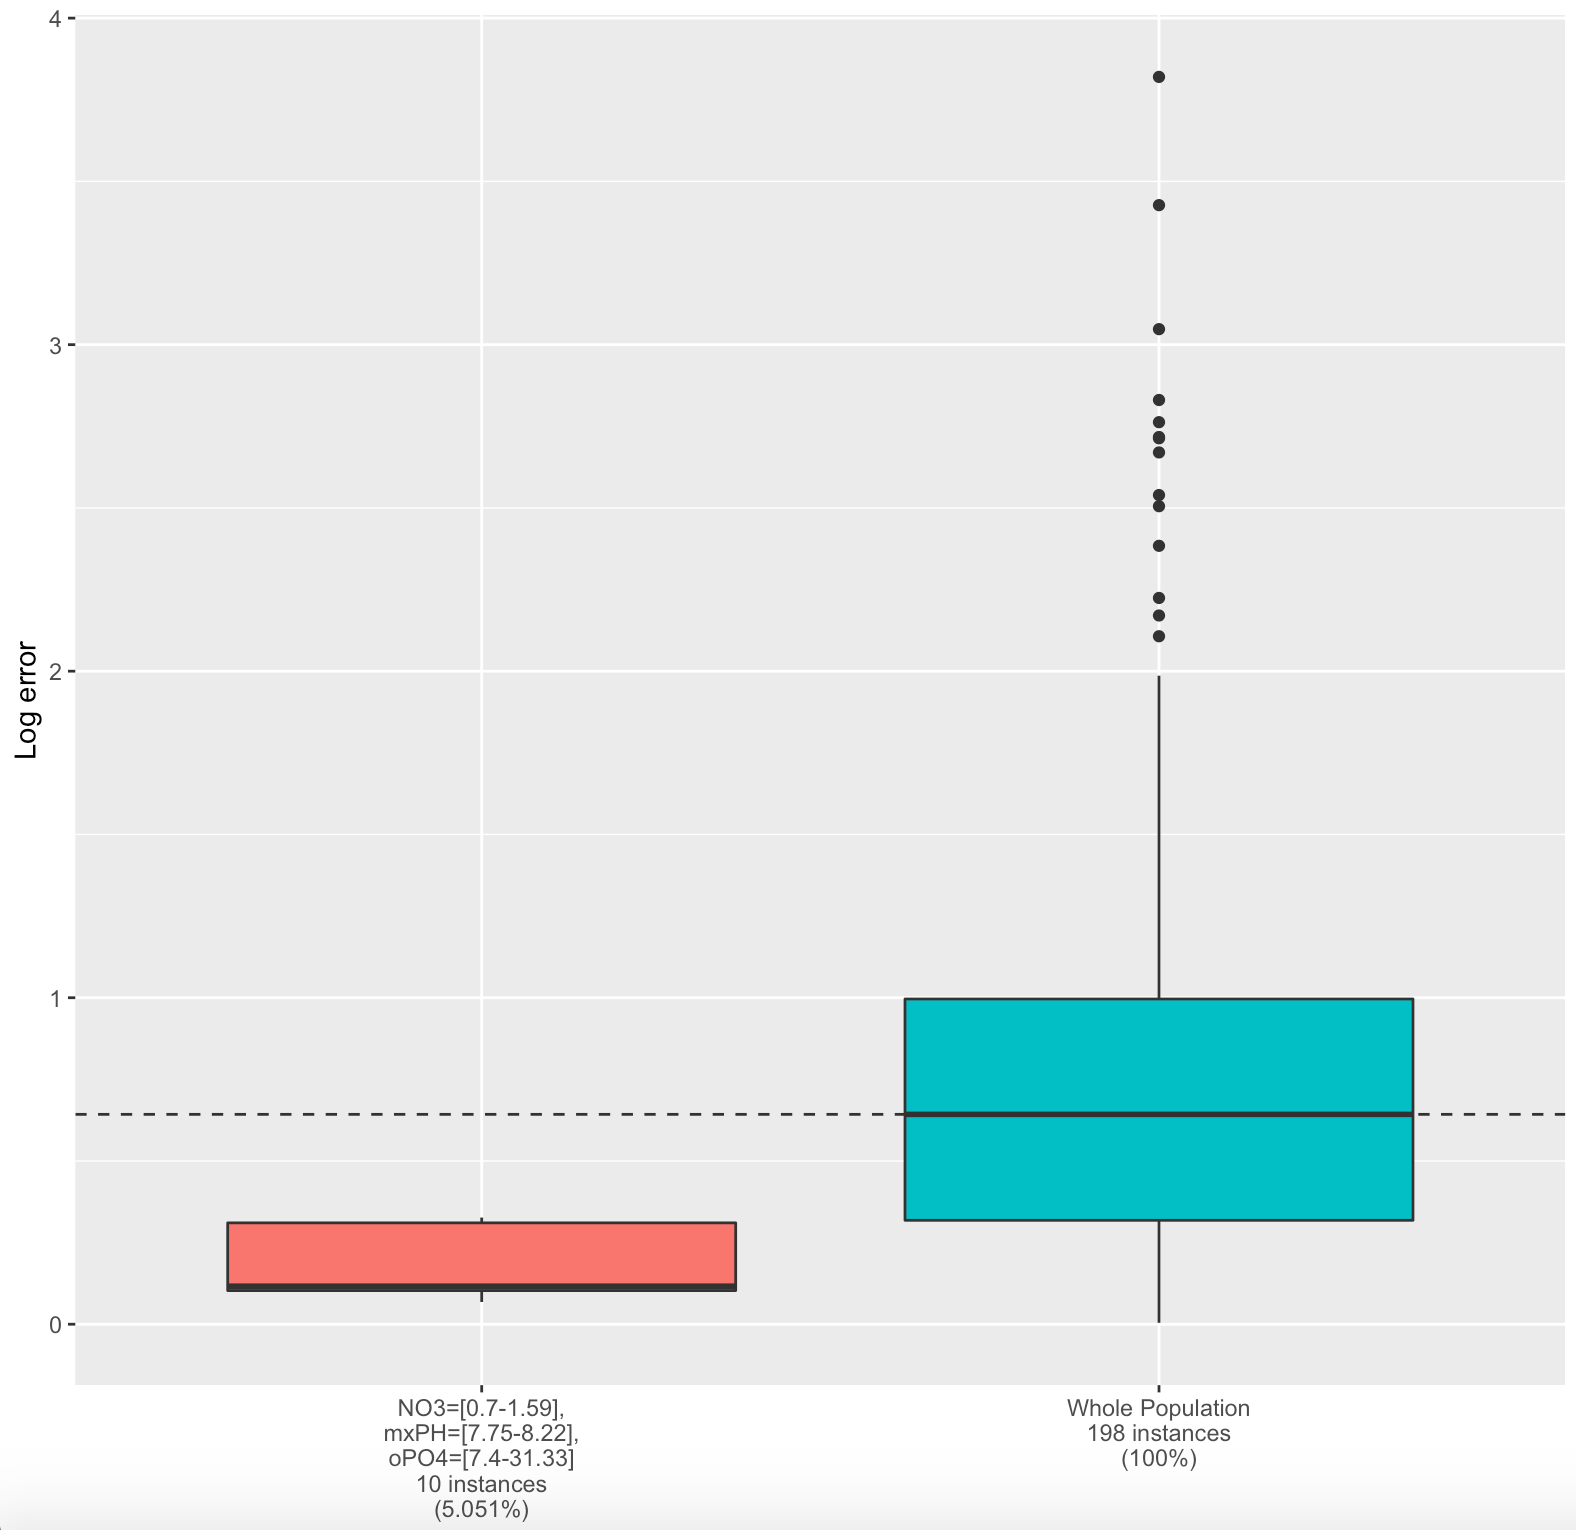
\includegraphics[width=0.97\linewidth]{/chpt_4/boxplot/single.png}
  \caption{Caption.} 
  \label{fig:subfigure_3}
\end{subfigure}
\caption{Caption.}
\label{fig:fig_2}
\end{figure}

\section{Summary}

Summary of the Chapter